\documentclass{beamer}\usepackage[]{graphicx}\usepackage[]{xcolor}
% maxwidth is the original width if it is less than linewidth
% otherwise use linewidth (to make sure the graphics do not exceed the margin)
\makeatletter
\def\maxwidth{ %
  \ifdim\Gin@nat@width>\linewidth
    \linewidth
  \else
    \Gin@nat@width
  \fi
}
\makeatother

\definecolor{fgcolor}{rgb}{0.345, 0.345, 0.345}
\newcommand{\hlnum}[1]{\textcolor[rgb]{0.686,0.059,0.569}{#1}}%
\newcommand{\hlstr}[1]{\textcolor[rgb]{0.192,0.494,0.8}{#1}}%
\newcommand{\hlcom}[1]{\textcolor[rgb]{0.678,0.584,0.686}{\textit{#1}}}%
\newcommand{\hlopt}[1]{\textcolor[rgb]{0,0,0}{#1}}%
\newcommand{\hlstd}[1]{\textcolor[rgb]{0.345,0.345,0.345}{#1}}%
\newcommand{\hlkwa}[1]{\textcolor[rgb]{0.161,0.373,0.58}{\textbf{#1}}}%
\newcommand{\hlkwb}[1]{\textcolor[rgb]{0.69,0.353,0.396}{#1}}%
\newcommand{\hlkwc}[1]{\textcolor[rgb]{0.333,0.667,0.333}{#1}}%
\newcommand{\hlkwd}[1]{\textcolor[rgb]{0.737,0.353,0.396}{\textbf{#1}}}%
\let\hlipl\hlkwb

\usepackage{framed}
\makeatletter
\newenvironment{kframe}{%
 \def\at@end@of@kframe{}%
 \ifinner\ifhmode%
  \def\at@end@of@kframe{\end{minipage}}%
  \begin{minipage}{\columnwidth}%
 \fi\fi%
 \def\FrameCommand##1{\hskip\@totalleftmargin \hskip-\fboxsep
 \colorbox{shadecolor}{##1}\hskip-\fboxsep
     % There is no \\@totalrightmargin, so:
     \hskip-\linewidth \hskip-\@totalleftmargin \hskip\columnwidth}%
 \MakeFramed {\advance\hsize-\width
   \@totalleftmargin\z@ \linewidth\hsize
   \@setminipage}}%
 {\par\unskip\endMakeFramed%
 \at@end@of@kframe}
\makeatother

\definecolor{shadecolor}{rgb}{.97, .97, .97}
\definecolor{messagecolor}{rgb}{0, 0, 0}
\definecolor{warningcolor}{rgb}{1, 0, 1}
\definecolor{errorcolor}{rgb}{1, 0, 0}
\newenvironment{knitrout}{}{} % an empty environment to be redefined in TeX

\usepackage{alltt}
\usepackage{graphicx}
\usepackage{graphicx}
\usepackage{verbatim}
\usepackage{etoolbox}
\usepackage{everysel}
% \usepackage{enumitem}

%% This package allows text highlighting
\usepackage{soul}

%% This sets the theme of the presentation which controls
%% the formatting of the slides
\usetheme{Boadilla}

%% Turn off the navigation symbols
\setbeamertemplate{navigation symbols}{} 

%% Change the default itemize [ball]s to [circle]s
\setbeamertemplate{itemize items}[circle]

%% Change the default enumerate [ball]s to plain text
\setbeamertemplate{enumerate items}[default]

%% Load the enumitem package and ensure it works nicely with beamer
% \setitemize{label=\usebeamerfont*{itemize item}
%   \usebeamercolor[fg]{itemize item}
%   \usebeamertemplate{itemize item}}
% \setenumerate{label=\usebeamerfont*{enumerate item}
%   \usebeamercolor[fg]{enumerate item}
%   \usebeamertemplate{enumerate item}}

%% Set the author block so STATS 201/8 appears on every
\author{STATS 201/8}

%% Clear the date block
\date{}


\setbeamercolor{title}{bg=blue!40}
\setbeamerfont{title}{size=\LARGE,series=\bfseries}

%%Sectioning commands
\setbeamercolor{section title}{bg=blue!20}
\setbeamerfont{section title}{size=\large}

\setbeamertemplate{section page}{%
    \begingroup
        \begin{beamercolorbox}[sep=10pt,center,rounded=true,shadow=true]{section title}
        \usebeamerfont{section title}Section~\thechapter.\thesection \newline \insertsection\par
        \end{beamercolorbox}
		\vfill
    \endgroup
}

\newcommand{\BeginSection}[1]{\section{#1} \frame{\sectionpage}}
%\AtBeginSection[]{%
%    \begin{frame}
%        \sectionpage
%    \end{frame}
%}


%% This makes all equations blue
\AtBeginEnvironment{equation*}{\color{blue}}
\AtBeginEnvironment{align*}{\color{blue}}
\everymath{\color{blue}}

%% This puts a 0 point space between paragraphs, means we don't need to use vspace, or list environments if 
%% we don't want to
\setlength{\parskip}{0pt}


%% Russell: removes spaces after R input/output?
\setlength{\topsep}{0.5mm}

%% David: In addition to Russel's command to remove spaces after R input/output, these commands remove the space between R input/output.
%% Stackoverflow link: https://stackoverflow.com/questions/35734525/reduce-space-between-code-chunks-and-code-output-in-rmarkdown-beamer-presentatio
%% \setlength{\OuterFrameSep}{-2pt}
\makeatletter
\preto{\@verbatim}{\topsep=-1pt \partopsep=-1pt }
\makeatother

%% Some useful colors
\definecolor{darkgreen}{rgb}{0.176,0.486,0.031}
\definecolor{redbrown}{HTML}{950605}
\definecolor{darkred}{HTML}{d80605}


%% nice little macro for changing the font of R code
\newcommand{\rcode}[1]{\protect{\color{darkgreen}\texttt{#1}}}

%% macro for bold blue italics
\newcommand{\blueBoldEmph}[1]{{\color{blue}\textbf{\emph{#1}}}}

% ~iid macro
\newcommand{\iid }{\stackrel{iid}{\sim}}

%% Macro for t-test amd P-value
\newcommand{\ttest}{\emph{t}-test}
\newcommand{\pval}{\emph{P}-value}

%% Statistics operators 
\DeclareMathOperator{\Bias}{Bias}
\DeclareMathOperator{\Cov}{Cov}
\DeclareMathOperator*{\Cor}{Cor}
\DeclareMathOperator{\E}{E}
\DeclareMathOperator{\MSE}{MSE}
\DeclareMathOperator{\Odds}{Odds}
\DeclareMathOperator{\OR}{OR}
\DeclareMathOperator{\PMSE}{PMSE}
\DeclareMathOperator{\sd}{sd}
\DeclareMathOperator{\se}{se}
\DeclareMathOperator*{\Var}{Var}
\DeclareMathOperator{\logit}{logit}

%% Should see if can make this a mathop
\newcommand{\comb}[2]{\mbox{$\big(_{#2}^{#1}\big)$}}




\setlength{\parskip}{9pt}
\IfFileExists{upquote.sty}{\usepackage{upquote}}{}
\begin{document}
\newcommand{\thechapter}{2}


\title{Chapter 2: \\ The basics of simple linear regression}
\institute{University of Auckland}

\begin{frame}
\titlepage
\end{frame}

\begin{frame}[t]
\frametitle{Learning outcomes}
In this chapter you will learn about:
\begin{center}
\vspace{6pt}
\begin{minipage}{0.9\textwidth}
  \begin{itemize}
  \item Fitting the linear model by minimizing the sum of the squared residuals
  \item The standard assumptions of the linear model
  \item Model checks of these assumptions  --  independence, EOV and normality
  \item Checking for points of undue influence using \rcode{cooks20x}
  \item Making inference from your model (provided the assumptions check out)
  \item Confidence intervals for population-level inference
  \item Prediction intervals for individual-level inference
  \item A recipe for subsequent analyses and relevant \rcode{R}-code.
  \end{itemize}
\end{minipage}
\end{center}
\end{frame}




%%%%%%%%%%%%%%%%%%%%%%%%%%%%%%%%%%%%%%%%%%%%%%%%%%%%%%%%%%%%%%%%%%%%%%%%%%%%%%%%%%%%%%%%%%%
\BeginSection{Fitting the linear model by minimizing the sum of the squared residuals}
%%%%%%%%%%%%%%%%%%%%%%%%%%%%%%%%%%%%%%%%%%%%%%%%%%%%%%%%%%%%%%%%%%%%%%%%%%%%%%%%%%%%%%%%%%%



\begin{frame}[fragile,t]
\frametitle{The fitted model}
\framesubtitle{Fitted values and residuals}
Recall, our simple linear model is $y_i=\beta_0+\beta_1 x_i+\varepsilon_i$, where $\beta_0$, $\beta_1$ and $\varepsilon_i$ are all unknown. After we fit this model to data, we can write
\begin{align*}
y_i &=\hat{y_i} + r_i \\
&= \left(\hat{\beta}_0+\hat{\beta}_1x_i\right)+r_i
\end{align*}
The two components in the above formulation are: 
\begin{itemize}
\item The fitted (or predicted) value, $\hat{y}_i=\hat{\beta}_0+\hat{\beta}_1 x_i$. 
This is the estimated value of $E[Y_i|x_i]=\beta_0+\beta_1 x_i$.
\item And what is left over, the {\bf residual}, $r_i$, the estimated value of $\varepsilon_i$. 
\end{itemize}

A natural question is: How are $\hat{\beta}_0$ and $\hat{\beta}_1$ estimated from the data???

We will answer this question in the next few slides in the context of our exam vs test mark example.
\end{frame}



\begin{frame}[fragile]
\frametitle{Exam vs.\ Test marks\ldots}
\framesubtitle{Fitted values and residuals\ldots}

First, let us examine one student in particular -- student (observation) number $i=21$.
\begin{knitrout}\scriptsize
\definecolor{shadecolor}{rgb}{0.969, 0.969, 0.969}\color{fgcolor}\begin{kframe}
\begin{alltt}
\hlstd{> }\hlcom{## Student # 21}
\hlstd{> }\hlstd{Stats20x.df} \hlkwb{=} \hlkwd{read.table}\hlstd{(}\hlstr{"Data/STATS20x.txt"}\hlstd{,} \hlkwc{header}\hlstd{=}\hlnum{TRUE}\hlstd{)}
\hlstd{> }\hlstd{Stats20x.df[}\hlnum{21}\hlstd{,]}
\end{alltt}
\begin{verbatim}
   Grade Pass Exam Degree Gender Attend Assign Test  B  C MC Colour Stage1
21     A  Yes   77    BSc Female     No   16.4 12.7 15 18 22  Green      A
   Years.Since Repeat
21         0.5     No
\end{verbatim}
\begin{alltt}
\hlstd{> }\hlstd{examtest.fit} \hlkwb{=} \hlkwd{lm}\hlstd{(Exam} \hlopt{~} \hlstd{Test,} \hlkwc{data} \hlstd{= Stats20x.df)}
\end{alltt}
\end{kframe}
\end{knitrout}

She got 12.7 out of 20 for the \rcode{Test} and 77 for an exam mark.
Again if we say $y=\rcode{Exam}$ and $x=\rcode{Test}$ then for her: 
$y_{21}=77$  and $x_{21} = 12.7$.

\end{frame}


\begin{frame}[fragile]
\frametitle{Exam vs.\ Test marks\ldots}
\framesubtitle{Fitted values and residuals\ldots}

According to the fitted model her fitted/predicted value is
\[
\hat{y}_{21}=\hat{\beta}_0+\hat{\beta}_1x_{21} =9.08+3.79\times 12.7=57.1657
\]
so she seems to have done better than predicted!
The residual value for her is:
\[
r_{21}={y}_{21}-\hat{y}_{21}=77-57.1657=19.8343.
\]
These calculations are done for all $i=1,2,\ldots, n=146$ students.

\rcode{R} did these calculations when we created the \rcode{lm} object \rcode{examtest.fit}.
Here is how to extract this information for student $i=21$:
\begin{knitrout}\scriptsize
\definecolor{shadecolor}{rgb}{0.969, 0.969, 0.969}\color{fgcolor}\begin{kframe}
\begin{alltt}
\hlstd{> }\hlkwd{resid}\hlstd{(examtest.fit)[}\hlnum{21}\hlstd{]}
\end{alltt}
\begin{verbatim}
     21 
19.8343 
\end{verbatim}
\begin{alltt}
\hlstd{> }\hlkwd{fitted}\hlstd{(examtest.fit)[}\hlnum{21}\hlstd{]}
\end{alltt}
\begin{verbatim}
     21 
57.1657 
\end{verbatim}
\end{kframe}
\end{knitrout}

\end{frame}

%Page 22
\begin{frame}[fragile]
\frametitle{Exam vs.\ Test marks\ldots}
\framesubtitle{Fitted values and residuals\ldots}
Here is her observed value $y_{21}$  - ({\color{red}red} point) and her associated fitted\footnote{We frequently use these expressions ``fitted" values and ``predicted" values interchangeably -- with some exceptions -- more later!}  value $\hat{y}_{21}$ marked ({\color{blue}blue} point).




\begin{figure}
  \centering
  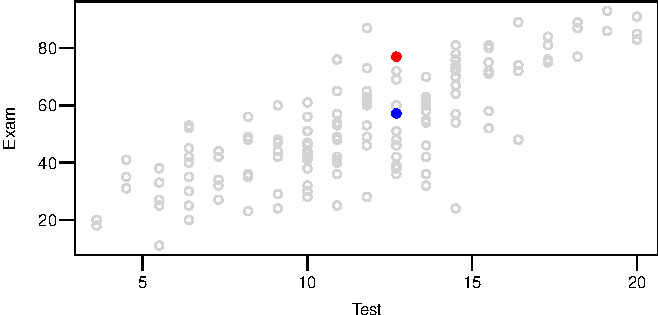
\includegraphics{figure/RC-H02-005}
\end{figure}

\end{frame}


\begin{frame}[fragile]
\frametitle{Exam vs.\ Test marks\ldots}
\framesubtitle{Fitted values and residuals\ldots}

In greater detail:




\begin{figure}
  \centering
  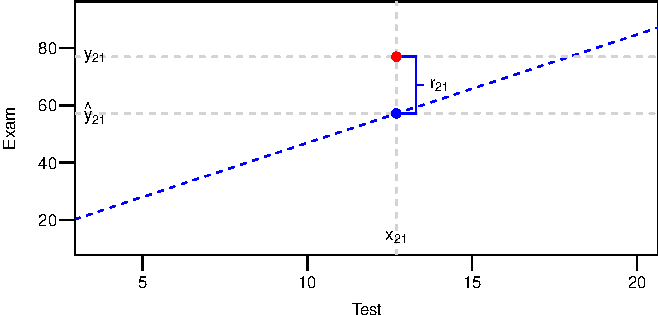
\includegraphics{figure/RC-H02-007}
\end{figure}

The residual is the vertical distance between the observed exam mark and the predicted exam mark.

\end{frame}


\begin{frame}[fragile]
\frametitle{Calculating $\hat{\beta}_0$ and $\hat{\beta}_1$}
\framesubtitle{Least squares}
The estimates, $\hat{\beta}_{0}$ and  $\hat{\beta}_{1}$, are obtained as the values
of $\beta_0$ and $\beta_1$ that minimise the least squares equation:
\[
\sum_{i=1}^{n}\varepsilon_{i}^2=\sum_{i=1}^{n}(y_i-\beta_0-\beta_1 x_i )^2.
\]

This minimized value is
\[
\sum_{i=1}^{n}(y_i-\hat{\beta}_0-\hat{\beta}_1 x_i )^2 = \sum_{i=1}^{n}r_{i}^2.
\]

In  effect this minimises the sum (over all observations) of the squared residuals.
Hence the name \textbf{``least squares"}.

\medskip This can be solved using a bit of calculus and/or linear algebra taught in, say, MATHS 208. A bit more detail is also given in STATS 330.

\end{frame}


\begin{frame}[fragile]
\frametitle{Exam vs.\ Test marks\ldots}
\framesubtitle{Residual sum of squares and $R^2$.}
Recall that we've already seen the sum of the squared residuals from the fitted model,
$\sum_{i=1}^{n}r_{i}^2$. It is the residual sum of squares (RSS). 
It can be calculated using the \rcode{R} code

\begin{knitrout}\scriptsize
\definecolor{shadecolor}{rgb}{0.969, 0.969, 0.969}\color{fgcolor}\begin{kframe}
\begin{alltt}
\hlstd{> }\hlkwd{sum}\hlstd{(}\hlkwd{resid}\hlstd{(examtest.fit)}\hlopt{^}\hlnum{2}\hlstd{)}
\end{alltt}
\begin{verbatim}
[1] 20901.08
\end{verbatim}
\end{kframe}
\end{knitrout}
\medskip

Similarly, the RSS of the null model is the total sum of squares,
\begin{knitrout}\scriptsize
\definecolor{shadecolor}{rgb}{0.969, 0.969, 0.969}\color{fgcolor}\begin{kframe}
\begin{alltt}
\hlstd{> }\hlkwd{sum}\hlstd{(}\hlkwd{resid}\hlstd{(}\hlkwd{lm}\hlstd{(Exam}\hlopt{~}\hlnum{1}\hlstd{,}\hlkwc{data}\hlstd{=Stats20x.df))}\hlopt{^}\hlnum{2}\hlstd{)}
\end{alltt}
\begin{verbatim}
[1] 50585.78
\end{verbatim}
\end{kframe}
\end{knitrout}
\medskip

Note that, compared to the null model, 
the RSS is reduced by 59\% when test score is in the model.
That is, the $R^2$ of \rcode{examtest.fit} is $0.59$.
\end{frame}



%%%%%%%%%%%%%%%%%%%%%%%%%%%%%%%%%%%%%%%%%%%%%%%%%%%%%%%%%%%%%%%%%%%%%%%%%%%%%%%%%%%%%%%%%%%
\BeginSection{The standard assumptions of the linear model}
%%%%%%%%%%%%%%%%%%%%%%%%%%%%%%%%%%%%%%%%%%%%%%%%%%%%%%%%%%%%%%%%%%%%%%%%%%%%%%%%%%%%%%%%%%%




\begin{frame}[fragile]
\frametitle{General assumptions of all linear models}

In this chapter we will discuss the set of assumptions we make when using linear models for inference. 

\medskip

We will show how these assumptions relate specifically to the simple linear model we have seen so far.

\medskip

However, whatever we learn here is also applicable to the other types of linear models that we will encounter.

\medskip

In later chapters we will encounter situations where these assumptions cannot hold. However, we will find appropriate ways to still use a linear model.

\end{frame}


\begin{frame}[fragile,t]
\frametitle{General assumptions of all linear models\ldots}
\framesubtitle{The underlying assumptions}
Let us state and examine our model a little more carefully.

Our simple linear regression model is
\[
y_i=\beta_0+\beta_1 x_i+\varepsilon_i, \ \ \varepsilon_i \iid N(0, \sigma^2)
\]
where each observation is indexed\footnote{The indexing variable $i$ is simply a labelling device. So, in out test vs exam example where $y=\rcode{Exam}$ and $x=\rcode{Test}$ we are saying that each student (observation) has a label associated with them from $i=1, 2, 3\ldots, n=146$.} with a subscript $i$ and $iid$ stands for  \textbf{i}ndependently and \textbf{i}dentically \textbf{d}istributed.

The above model formula is saying that
\[
\varepsilon_i = y_i - \beta_0+\beta_1 x_i 
\]
is distributed according to
\[
\varepsilon_i \iid N(0, \sigma^2)
\]
\end{frame}



\begin{frame}[fragile]
\frametitle{General assumptions of all linear models\ldots}
\framesubtitle{The underlying assumptions\ldots}
The model assumptions are with regard to the random variability component
\[
\varepsilon_i \iid N(0, \sigma^2)
\]
\vspace{-2em}

\begin{enumerate}
\item \textbf{Independent:} We require every observation to be independent of every other observation.\footnote{If the $y_i$ are independent then so too are the $\varepsilon_i$.} This requires that the data are collected in an appropriate manner, such as a simple random sample. In practice, achieving truely independent data can be challenging.
\smallskip

\item \textbf{Identically} distributed: The $\varepsilon_i$ must all come from the same distribution, and this distribution must have mean of 0. All $\varepsilon_i$ must necessarily have the same variance, which we refer to as the equality of variance, (\textbf{EOV}), assumption. 
\smallskip

\item \textbf{Distributed} normally: The $\varepsilon_i$ must be from a normal distribution, at least approximately.
\end{enumerate}

\end{frame}




\begin{frame}[fragile]
\frametitle{Model assumptions}
\framesubtitle{Exam vs.\ Test marks}
Let's consider the underlying assumptions about $\varepsilon_i \iid N(0,\sigma^2)$ in the context of our ongoing example.  

In decreasing order of importance:

\begin{itemize}
\item \textbf{Independent:} It was an invigilated exam so the variabilities in the exam scores of students should all be independent. 

\item \textbf{Identically} distributed: If the {\bf linear} relationship is reasonable then
\begin{itemize} 
\item  The residuals\footnote{Recall, the residuals $r_i$ are our estimates of $\varepsilon_i$} will be randomly scattered around 0.
\item The residuals should have roughly constant scatter, i.e., satisfy the equality Of Variance (EOV) requirement.
\end{itemize}

\item \textbf{Distributed} normally: The residuals should be (at least roughly) normally distributed -- only check this if the first two assumptions are validated.
\end{itemize}

\end{frame}


\begin{frame}
\frametitle{Very important aside!}
\begin{Large}
If the linear model assumptions do not hold, it \textbf{does not} mean we cannot do anything. 
\end{Large}
\bigskip

When assumptions are not satisfied there are often techniques that we can use to transform our data and/or model so that the assumptions {\bf will} be satisfied.  We will see some of these techniques later in this course.
\bigskip

There are also other techniques that can ``free up'' some of the assumptions. For example, lack of independence in time series data is covered later in this course, and other techniques are seen in more advanced courses. 

\end{frame}



%%%%%%%%%%%%%%%%%%%%%%%%%%%%%%%%%%%%%%%%%%%%%%%%%%%%%%%%%%%%%%%%%%%%%%%%%%%%%%%%%%%%%%%%%%%
\BeginSection{Checks of model assumptions  --  independence, EOV and normality}
%%%%%%%%%%%%%%%%%%%%%%%%%%%%%%%%%%%%%%%%%%%%%%%%%%%%%%%%%%%%%%%%%%%%%%%%%%%%%%%%%%%%%%%%%%%


\begin{frame}[fragile]
\frametitle{EOV check: Plotting residuals vs fitted values}

Let us check the \textbf{EOV} assumption. 
We are assuming that what cannot be explained has random constant scatter about zero 
regardless of the fitted value. 


That is, for each fitted (or predicted) value we have a similar distribution for what cannot be explained. We can check this by looking at each fitted (predicted) value versus its associated residual value. 

Our fitted model is:
\[
y_i=\hat{y_i} + r_i= \left(\hat{\beta}_0+\hat{\beta}_1x_i\right)+r_i.
\]

It is useful to draw a scatter plot with $\hat{y_i}$ on the horizontal axis and $r_i$ on the vertical axis.


This is more generally known as a {\it residuals vs fitted values} plot.

\end{frame}


\begin{frame}[fragile]
\frametitle{Exam vs.\ Test marks\ldots}
\framesubtitle{EOV check: Plotting residuals vs fitted values\ldots}
Producing a scatter plot of residuals versus fitted values is easy\footnote{You can also use
the \rcode{s20x} function \rcode{eovcheck}, i.e., \rcode{eovcheck(exam.fit)}}. 

\begin{knitrout}\scriptsize
\definecolor{shadecolor}{rgb}{0.969, 0.969, 0.969}\color{fgcolor}\begin{kframe}
\begin{alltt}
\hlstd{> }\hlkwd{plot}\hlstd{(examtest.fit,} \hlkwc{which}\hlstd{=}\hlnum{1}\hlstd{)}
\end{alltt}
\end{kframe}
\end{knitrout}



\begin{figure}
  \centering
  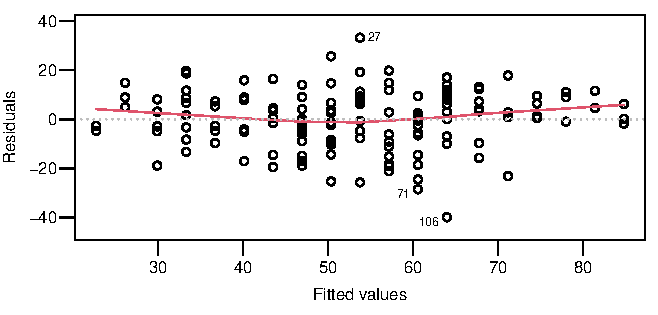
\includegraphics{figure/RC-H02-009}
\end{figure}

\end{frame}


\begin{frame}[fragile]
\frametitle{Exam vs.\ Test marks\ldots}
\framesubtitle{EOV check: Plotting residuals vs fitted values\ldots}
The above residual plot exhibits a patternless band of random points - this is to be expected since
the original scatter plot of the data had a straight line trend and
reasonably constant scatter: 

\begin{knitrout}\scriptsize
\definecolor{shadecolor}{rgb}{0.969, 0.969, 0.969}\color{fgcolor}\begin{kframe}
\begin{alltt}
\hlstd{> }\hlkwd{trendscatter}\hlstd{(Exam}\hlopt{~}\hlstd{Test,} \hlkwc{data} \hlstd{=Stats20x.df)}
\end{alltt}
\end{kframe}
\end{knitrout}



\begin{figure}
  \centering
  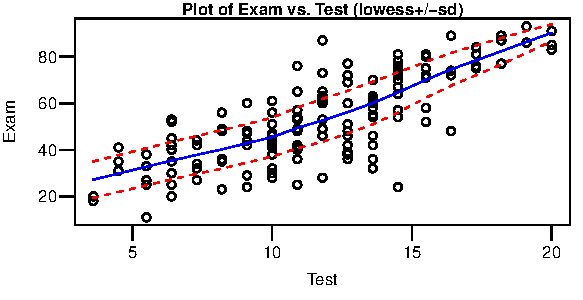
\includegraphics{figure/RC-H02-011}
\end{figure}

\end{frame}



\begin{frame}[fragile]
\frametitle{Exam vs.\ Test marks\ldots}
\framesubtitle{EOV check: Plotting residuals vs fitted values\ldots}

The plot of residuals versus fitted values confirms reasonably constant scatter (variance). 

Note that at the high end of exam/test scores there are not that many students (unfortunately!) so the relative lack of spread is not surprising. 

\end{frame}


\begin{frame}[fragile]
\frametitle{Exam vs.\ Test marks\ldots}
\framesubtitle{Normality of residuals}

Having validated the \textbf{EOV} assumption, let us perform the normality check 
by examining the residuals.  
%\textbf{Note } do not check normality if \textbf{EOV} as it is essentially meaningless. 
We have written a function in \rcode{R} called \rcode{normcheck} to do just that:

\begin{knitrout}\scriptsize
\definecolor{shadecolor}{rgb}{0.969, 0.969, 0.969}\color{fgcolor}\begin{kframe}
\begin{alltt}
\hlstd{> }\hlkwd{normcheck}\hlstd{(examtest.fit)}
\end{alltt}
\end{kframe}
\end{knitrout}



\begin{figure}
  \centering
  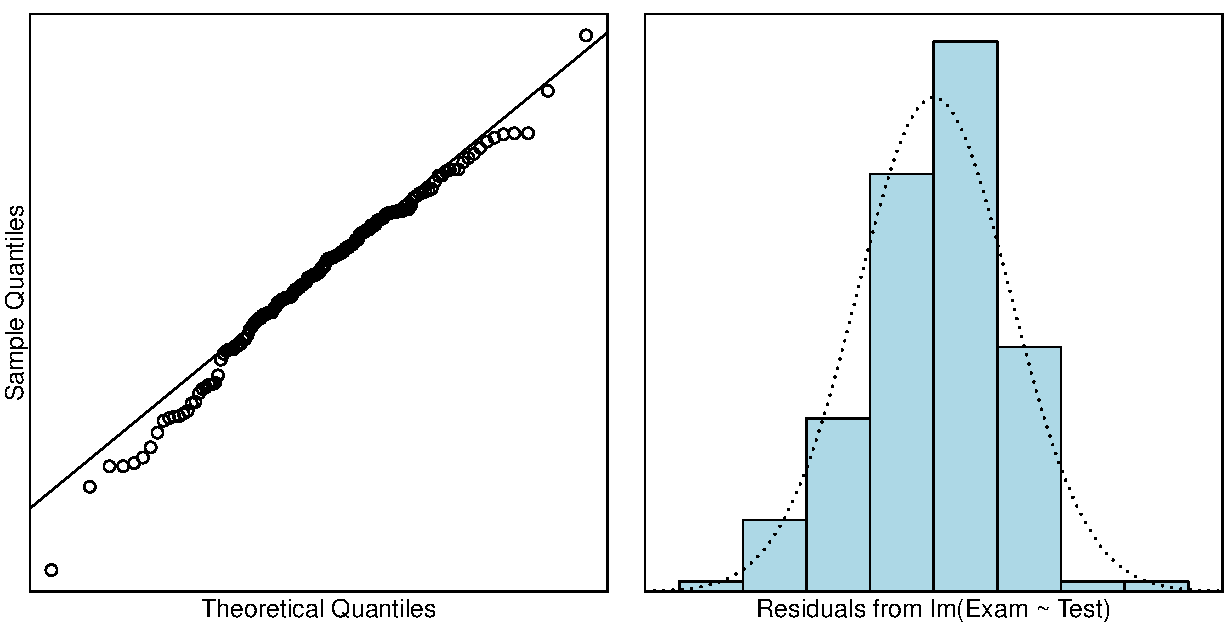
\includegraphics[scale=0.5]{figure/RC-H02-015}
\end{figure}
 
\end{frame}


\begin{frame}[fragile]
\frametitle{Exam vs.\ Test marks\ldots}
\framesubtitle{Normality of residuals}
The histogram of the residuals (right plot) tells us we are okay since it closely matches
a normal bell-shaped curve (shown by the dashed line).
\medskip

The normal quantile-quantile-plot (\rcode{qqplot}) in the left hand plot gives further insight.  In this example, the 146 theoretical quantile values on the x-axis can be regarded as the values that would give a near perfect bell-shaped histogram (i.e., would best match the dashed bell-shaped curve in the right hand plot). Ideally, our residuals should match these theoretical quantiles and lie approximately on the straight line shown on the \rcode{qqplot}.
\medskip

It can be difficult to judge if a qq-plot is sufficiently close to a straight line or not. Some intuition can be gained by seeing how the qq-plot looks when the assumptions are satisfied, as shown on the next slide. In comparison, the above qq-plot does look a little atypical, but not enough to cause major concerns.
\end{frame}



\begin{frame}[fragile]
\frametitle{Exam vs.\ Test marks\ldots}
\framesubtitle{qq-plot intuition}

\begin{knitrout}\scriptsize
\definecolor{shadecolor}{rgb}{0.969, 0.969, 0.969}\color{fgcolor}\begin{kframe}
\begin{alltt}
\hlstd{> }\hlkwa{for}\hlstd{(i} \hlkwa{in} \hlnum{1}\hlopt{:}\hlnum{6}\hlstd{) \{}
\hlstd{+ }  \hlstd{y}\hlkwb{=}\hlkwd{rnorm}\hlstd{(}\hlnum{146}\hlstd{)}
\hlstd{+ }  \hlkwd{qqnorm}\hlstd{(}\hlkwd{resid}\hlstd{(}\hlkwd{lm}\hlstd{(y}\hlopt{~}\hlnum{1}\hlstd{)),}\hlkwc{main}\hlstd{=}\hlstr{""}\hlstd{);} \hlkwd{abline}\hlstd{(}\hlnum{0}\hlstd{,}\hlnum{1}\hlstd{) \}}
\end{alltt}
\end{kframe}
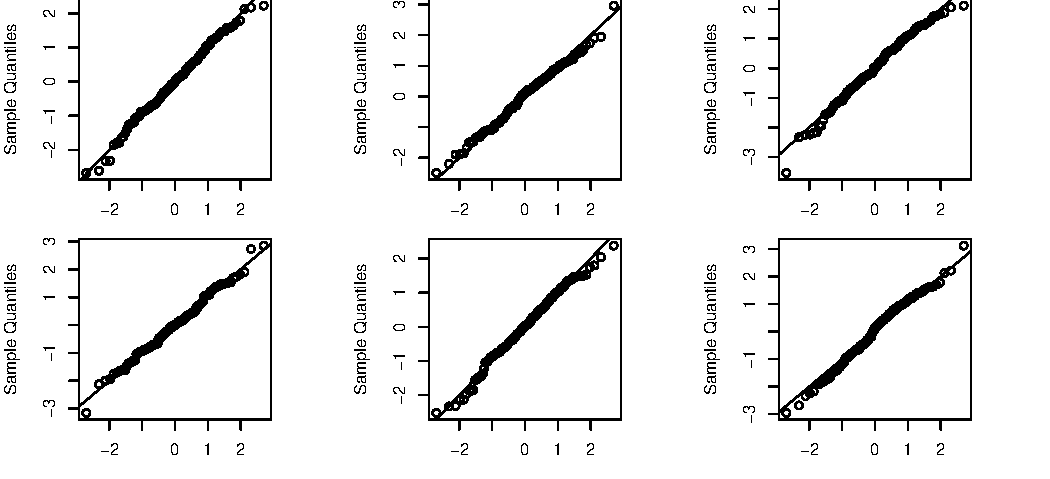
\includegraphics[width=\maxwidth]{figure/RC-H02-015b-1} 
\end{knitrout}

\end{frame}



\begin{frame}[fragile]
\frametitle{Exam vs.\ Test marks\ldots}
\framesubtitle{A further check: Influence}

Before we rush in and conclude that all is well, 
there is one other concern that we should investigate, namely \emph{influence}.\footnote{This is not a model assumption per se, but is a prudent model check.}

\bigskip

Essentially, we need to check whether the fit is highly influenced by any single
(or small group of) observation(s).

\end{frame}




%%%%%%%%%%%%%%%%%%%%%%%%%%%%%%%%%%%%%%%%%%%%%%%%%%%%%%%%%%%%%%%%%%%%%%%%%%%%%%%%%%%%%%%%%%%
\BeginSection{Checking for points of undue influence using \rcode{cooks20x}}
%%%%%%%%%%%%%%%%%%%%%%%%%%%%%%%%%%%%%%%%%%%%%%%%%%%%%%%%%%%%%%%%%%%%%%%%%%%%%%%%%%%%%%%%%%%



\begin{frame}[fragile]
\frametitle{Points of undue influence}


The fitted model is based on minimizing the sum of the squared residuals. Because of this, a single observation with a very large residual can have a big influence on the overall fit.
We can be misled if we assume all is fine when one (or several) data points are unduly influential, and perhaps of questionable validity.
\bigskip

Moreover, a data point can also be influential on the model fit by having an extreme $x$ value, since it can apply a lot of ``torque'' to the fit.

\end{frame}


\begin{frame}[fragile]
\frametitle{Exam vs.\ Test marks\ldots}
\framesubtitle{Points of undue influence\ldots}
To illustrate: Imagine a student had mistakenly been awarded 25 out of 20 in their \rcode{Test}, yet obtained just 5 in the final exam.
\bigskip

Here is some tricky \rcode{R} code to add this incorrect data point to our dataframe:
\begin{knitrout}\scriptsize
\definecolor{shadecolor}{rgb}{0.969, 0.969, 0.969}\color{fgcolor}\begin{kframe}
\begin{alltt}
\hlstd{> }\hlstd{n}\hlkwb{=}\hlkwd{nrow}\hlstd{(Stats20x.df)}
\hlstd{> }\hlcom{## Add extra point by repeating last observation, n(=146)}
\hlstd{> }\hlstd{Stats20xnew.df}\hlkwb{=}\hlstd{Stats20x.df[}\hlkwd{c}\hlstd{(}\hlnum{1}\hlopt{:}\hlstd{n,n),]}
\hlstd{> }\hlcom{## Replace with new test /Exam #'s}
\hlstd{> }\hlstd{Stats20xnew.df[n}\hlopt{+}\hlnum{1}\hlstd{,}\hlkwd{c}\hlstd{(}\hlstr{"Test"}\hlstd{,} \hlstr{"Exam"}\hlstd{)]}\hlkwb{=}\hlkwd{c}\hlstd{(}\hlnum{25}\hlstd{,}\hlnum{5}\hlstd{)}
\hlstd{> }\hlcom{## Plot our new dataset}
\hlstd{> }\hlkwd{plot}\hlstd{(Exam}\hlopt{~} \hlstd{Test,} \hlkwc{data}\hlstd{=Stats20xnew.df)}
\hlstd{> }\hlcom{## Mark our new observation}
\hlstd{> }\hlkwd{points}\hlstd{(}\hlnum{25}\hlstd{,}\hlnum{5}\hlstd{,}\hlkwc{pch}\hlstd{=}\hlnum{19}\hlstd{,}\hlkwc{col}\hlstd{=}\hlstr{"red"}\hlstd{)}
\end{alltt}
\end{kframe}
\end{knitrout}
\end{frame}


\begin{frame}[fragile]
\frametitle{Exam vs.\ Test marks\ldots}
\framesubtitle{Points of undue influence\ldots}


\begin{figure}
  \centering
  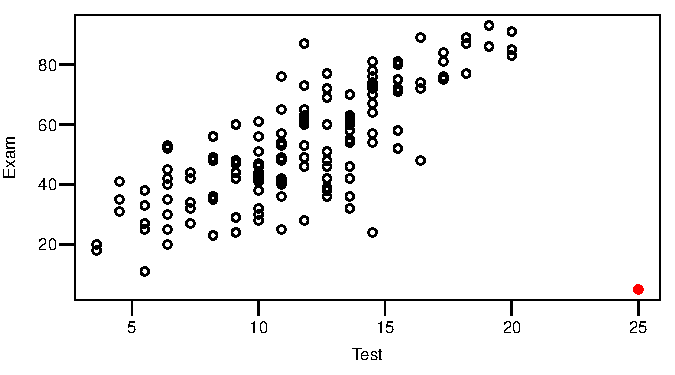
\includegraphics{figure/RC-H02-017}
\end{figure}

The bogus student is shown on the plot as the {\color{red}red} point!

\end{frame}

\begin{frame}[fragile]
\frametitle{Exam vs.\ Test marks\ldots}
\framesubtitle{Points of undue influence\ldots}
Here is the new model fitted to the altered data.
\begin{knitrout}\scriptsize
\definecolor{shadecolor}{rgb}{0.969, 0.969, 0.969}\color{fgcolor}\begin{kframe}
\begin{alltt}
\hlstd{> }\hlstd{examtest.fit2}\hlkwb{=}\hlkwd{lm}\hlstd{(Exam}\hlopt{~}\hlstd{Test,} \hlkwc{data}\hlstd{=Stats20xnew.df)}
\hlstd{> }\hlkwd{coef}\hlstd{(}\hlkwd{summary}\hlstd{(examtest.fit2))}
\end{alltt}
\end{kframe}
\end{knitrout}
\begin{knitrout}\scriptsize
\definecolor{shadecolor}{rgb}{0.969, 0.969, 0.969}\color{fgcolor}\begin{kframe}
\begin{verbatim}
             Estimate Std. Error   t value     Pr(>|t|)
(Intercept) 15.237389  3.7171579  4.099204 6.875383e-05
Test         3.200551  0.3022693 10.588407 9.162607e-20
\end{verbatim}
\end{kframe}
\end{knitrout}
Compare this to the original fit:
\begin{knitrout}\scriptsize
\definecolor{shadecolor}{rgb}{0.969, 0.969, 0.969}\color{fgcolor}\begin{kframe}
\begin{alltt}
\hlstd{> }\hlkwd{coef}\hlstd{(}\hlkwd{summary}\hlstd{(examtest.fit))}
\end{alltt}
\begin{verbatim}
            Estimate Std. Error   t value     Pr(>|t|)
(Intercept) 9.084463  3.2204410  2.820876 5.465681e-03
Test        3.785924  0.2647333 14.300897 1.985079e-29
\end{verbatim}
\end{kframe}
\end{knitrout}


Note how $\hat{\beta_1}$ has changed from 3.79 to 3.20. This is a change of more than two standard errors (here, we are referring to the standard error from the original fit, 0.265).
\end{frame}


\begin{frame}[fragile]
\frametitle{Exam vs.\ Test marks\ldots}
\framesubtitle{Points of undue influence\ldots}
Here is the old model fitted line ({\color{blue}blue}) compared to this new model ({\color{red}red}). \\
\phantom{A space}


\begin{figure}
  \centering
  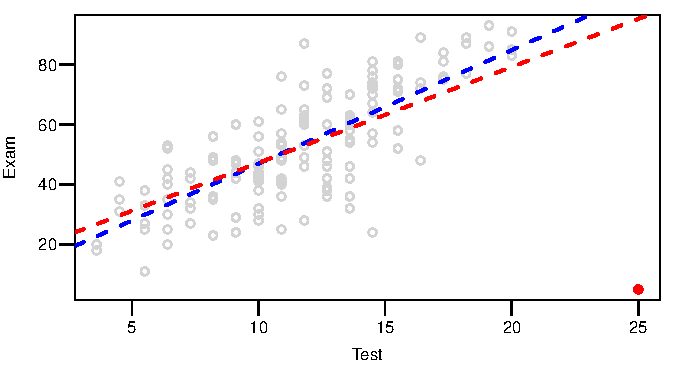
\includegraphics{figure/RC-H02-020}
\end{figure}

\end{frame}


\begin{frame}[fragile]
\frametitle{Exam vs.\ Test marks\ldots}

\framesubtitle{Points of undue influence\ldots}


How does this change predictions?

In this model we would make a prediction using the following estimates (to 2 d.p.).
 $\rcode{Exam}= 15.24 +3.20 \times\rcode{Test}$ compared to the old model estimates:
 $\rcode{Exam}= 9.08 +3.79 \times\rcode{Test}$

Our new vs.\ previous estimates are now (previous estimate in brackets):

\begin{itemize}
\item \rcode{Test = \phantom{0}0} then $\rcode{Exam}= 15.24 +3.20\times\rcode{\phantom{0}0} = 15.24$  (\phantom{0}9.08),
\item \rcode{Test = 10} then $\rcode{Exam}= 15.24 +3.20\times\rcode{10} = 47.24$ (46.94),
\item \rcode{Test = 20} then $\rcode{Exam}= 15.24 +3.20\times\rcode{20} = 79.25 $ (84.80).
\end{itemize}

Note that this has had a huge change for the extreme \rcode{Test} scores -- for those who got 0 in the \rcode{Test} we predict a higher mark than before and those who got a 20 (out of 20) get a lower predicted mark than before. 
\end{frame}


\begin{frame}[fragile]
\frametitle{Identifing points of undue influence}

The addition of student 147 has drastically changed our fitted model and its predictions. This studend is so atypical of the other 146 students that we should exclude them from the analysis. In this case it is clearly a data entry mistake, but in practice it is not always so obvious.

\bigskip \bigskip
We've seem that to determine whether an observation is influential we need to remove it from the dataset and refit the model. This can be a lot of work when there a lot of observations. The Cook's distance uses linear algebra to avoid this work. 
\end{frame}


\begin{frame}[fragile]
\frametitle{Identifing points of undue influence\ldots}
\framesubtitle{Cook's distance}

The following Cook's distance plot gives the influence of all 147 observations in the altered dataframe. Student 147 dominates this plot and is clearly identified as being highly influential.

\begin{knitrout}\scriptsize
\definecolor{shadecolor}{rgb}{0.969, 0.969, 0.969}\color{fgcolor}\begin{kframe}
\begin{alltt}
\hlstd{> }\hlkwd{cooks20x}\hlstd{(examtest.fit2)}
\end{alltt}
\end{kframe}
\end{knitrout}



\begin{figure}
  \centering
  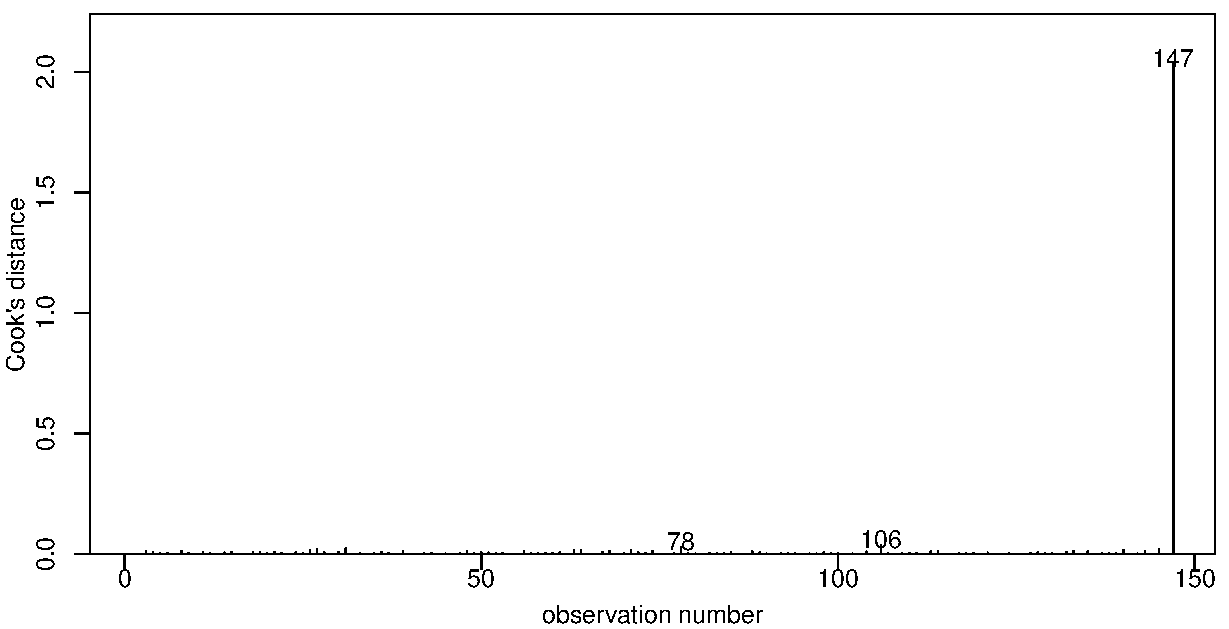
\includegraphics[scale=0.5]{figure/RC-H02-023}
\end{figure}

\end{frame}


\begin{frame}[fragile]
\frametitle{Identifing points of undue influence\ldots}

\medskip
As a rough ``rule of thumb"\footnote{\textbf{A rule of thumb} is a principle with broad application that is not intended to be strictly accurate or reliable for every situation. It is an easily learned and easily applied procedure for approximately calculating or recalling some value, or for making some determination. Thanks Wikipedia.},
an observation is deemed to be influential if:
\begin{itemize}
\item Removal of the observation changes any estimated parameter value by more than one standard error, or
\item Its Cook's distance is greater than 0.4.
\end{itemize}

In STATS 20x we'll use the above Cook's distance threshold of 0.4. (Be aware that other courses or texts may use other thresholds, and the threshold may depend on the number of observations.) 

Let us get back to the original fitted model and see what its Cook's distance plot looks like.

\end{frame}


\begin{frame}[fragile]
\frametitle{Exam vs.\ Test marks\ldots}
\framesubtitle{Identifing points of undue influence\ldots}

\begin{knitrout}\scriptsize
\definecolor{shadecolor}{rgb}{0.969, 0.969, 0.969}\color{fgcolor}\begin{kframe}
\begin{alltt}
\hlstd{> }\hlkwd{cooks20x}\hlstd{(examtest.fit)}
\end{alltt}
\end{kframe}
\end{knitrout}



\begin{figure}
  \centering
  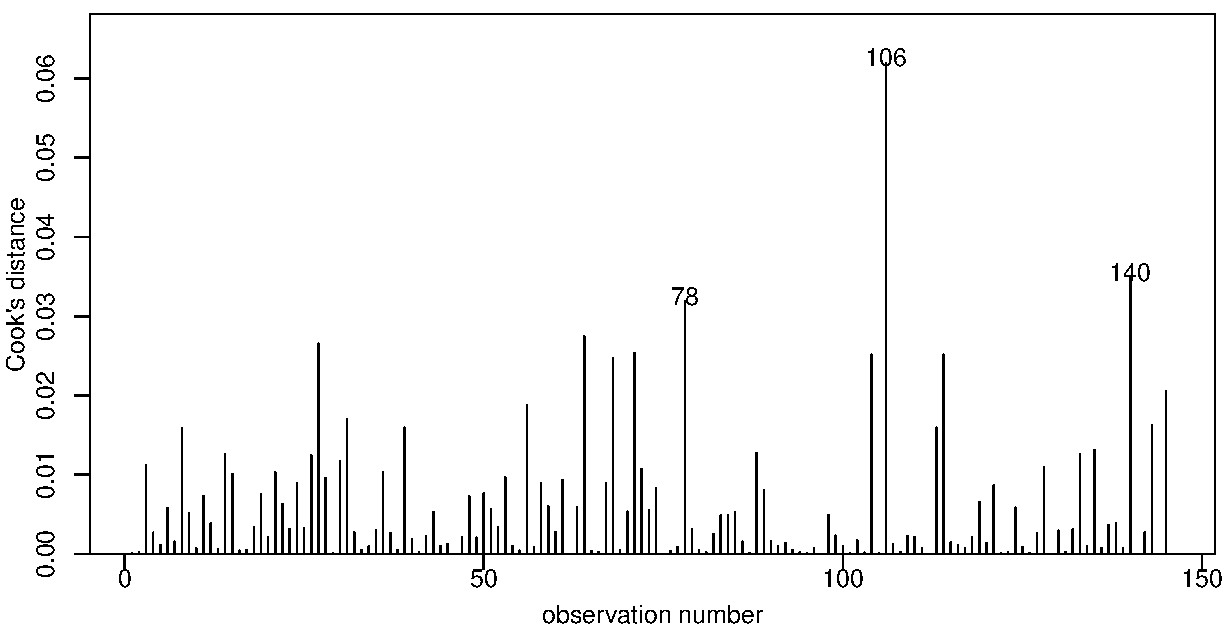
\includegraphics[scale=0.5]{figure/RC-H02-025}
\end{figure}

\end{frame}


\begin{frame}[fragile]
\frametitle{Exam vs.\ Test marks\ldots}
\framesubtitle{Validity of assumptions}

We may now conclude that we can (mostly) trust the output of our analysis as our underlying assumptions seem reasonable and we do not have any unduly influential data points.

\end{frame}



%%%%%%%%%%%%%%%%%%%%%%%%%%%%%%%%%%%%%%%%%%%%%%%%%%%%%%%%%%%%%%%%%%%%%%%%%%%%%%%%%%%%%%%%%%%
\BeginSection{Making inference from your model (provided the assumptions check out)}
%%%%%%%%%%%%%%%%%%%%%%%%%%%%%%%%%%%%%%%%%%%%%%%%%%%%%%%%%%%%%%%%%%%%%%%%%%%%%%%%%%%%%%%%%%%



\begin{frame}
\frametitle{Statistical properties of the fitted linear model}
Provided that {\bf all} of the assumptions of the linear model hold, it can be shown (see STATS 310) that $\hat{\beta}_0$ and $\hat{\beta}_1$ are normally distributed\footnote{That is, under repetition of the experiment that generated the data.} with expected values $\beta_0$ and $\beta_1$, respectively.
\bigskip

This means that the standard statistical techniques for making inference from normally distributed data can still be used.
\medskip

In particular, the t-statistic is used for testing hypotheses, and the t-multiplier for constructing confidence and prediction intervals.
\end{frame}
  

\begin{frame}[fragile]
\frametitle{Interpreting the output}
\framesubtitle{Testing for significant effects}

\begin{knitrout}\scriptsize
\definecolor{shadecolor}{rgb}{0.969, 0.969, 0.969}\color{fgcolor}\begin{kframe}
\begin{alltt}
\hlstd{> }\hlstd{examtest.fit} \hlkwb{=} \hlkwd{lm}\hlstd{(Exam} \hlopt{~} \hlstd{Test,} \hlkwc{data} \hlstd{= Stats20x.df)}
\hlstd{> }\hlkwd{summary}\hlstd{(examtest.fit)}
\end{alltt}
\end{kframe}
\end{knitrout}
\begin{knitrout}\scriptsize
\definecolor{shadecolor}{rgb}{0.969, 0.969, 0.969}\color{fgcolor}\begin{kframe}
\begin{verbatim}
Coefficients:
            Estimate Std. Error t value Pr(>|t|)    
(Intercept)   9.0845     3.2204   2.821  0.00547 ** 
Test          3.7859     0.2647  14.301  < 2e-16 ***
---
Residual standard error: 12.05 on 144 degrees of freedom
Multiple R-squared:  0.5868,	Adjusted R-squared:  0.5839 
F-statistic: 204.5 on 1 and 144 DF,  p-value: < 2.2e-16
\end{verbatim}
\end{kframe}
\end{knitrout}

So here we can see that the \pval{} associated with the \rcode{Test} variable is highly statistically significant \rcode{< 2e-16 ***}.\footnote{\rcode{2e-16} $ = 2\times 10^{-16}$, which is so small that we may just as well call it zero.}

Our underlying belief was that we could describe the relationship between exam mark and test mark using an increasing straight line. This belief has been confirmed.

\end{frame}


\begin{frame}[fragile]
\frametitle{Interpreting the output\ldots}
\framesubtitle{Testing for significant effects\ldots}

The null hypothesis is always that there is no effect. 
In this case, that there is no relationship between test score and exam score, i.e.,

$H_0$: there is no relationship between \rcode{Test} and \rcode{Exam}.

Or equivalently,

$H_0:\beta_1=0$, which is equivalent to saying that the data follow the \rcode{null} model $y=\beta_0+ \varepsilon$. 


We will pretend that the null hypothesis is true (i.e., our working model of an increasing linear relationship between test and exam is incorrect), at least until we get evidence to the contrary.
\medskip

This approach is known as the philosophy of ``falsification''. 
It is not the natural way we like to do things as humans, 
but is a great way to ensure we do not come to erroneous conclusions based on wishful thinking.

\end{frame}


\begin{frame}[fragile]
\frametitle{Interpreting the output\ldots}
\framesubtitle{Calculating the t value}


Under the null hypothesis we assume $\beta_1=0$ and compare this to the estimated value here of $\hat{\beta}_1=3.7859$.
As we are statisticians, we need to measure how precise this estimate is -- this is measured by the standard error: $se(\hat{\beta}_1)=0.2647$.

So under the assumption that $\beta_1=0$ we can say that our data tell us that we are 
\[
\frac{3.7859-0}{0.2647} =14.301
\]
standard deviations\footnote{The term ``standard error'' is used to refer to the standard deviation of an estimated value -- in this case the standard deviation of the estimated linear effect of \rcode{Test}.}  away from this value. 
You might recognize this as the $t$-statistic for testing $H_0:\beta_1=0$.
It is the \rcode{t value} in our output. 

Here, we conclude that our working model was reasonable. That is, it is unreasonable to assume that \rcode{Test} had no effect on \rcode{Exam} as the chances of fluking such a result is $<2\times 10^{-16}$.

\end{frame}


\begin{frame}[fragile]
\frametitle{Interpreting the output\ldots}
\framesubtitle{Null vs fitted models}

If $y=\rcode{Exam}$ and $x=\rcode{Test}$, then here are our fitted null (the {\color{red} red} line) and working (the {\color{blue} blue} line) models.

% Null model: $y=\beta_0+\varepsilon$ (red) versus 
% $y=\beta_0+\beta_1 x+\varepsilon$ (blue) where $\varepsilon\iid N(0,\sigma^2)$:



\begin{figure}
  \centering
  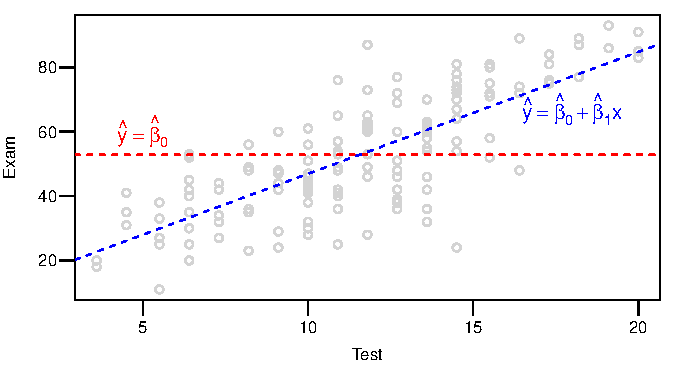
\includegraphics{figure/RC-H02-029}
\end{figure}

\end{frame}


\begin{frame}[fragile]
\frametitle{Statistical inference from our model}
\framesubtitle{Confidence intervals for effects}

We can also get confidence intervals for $\beta_1$ (and $\beta_0$ if need be) by:
\begin{knitrout}\scriptsize
\definecolor{shadecolor}{rgb}{0.969, 0.969, 0.969}\color{fgcolor}\begin{kframe}
\begin{alltt}
\hlstd{> }\hlkwd{confint}\hlstd{(examtest.fit)}
\end{alltt}
\begin{verbatim}
               2.5 %    97.5 %
(Intercept) 2.719020 15.449907
Test        3.262659  4.309189
\end{verbatim}
\end{kframe}
\end{knitrout}

Here we can say that, on average,  every increase in a student's test mark of 1 unit (out of 20) results in a 3.26 to 4.31 increase in the student's exam result.

\medskip
\textbf{Note}: the default setting is 95\% in \rcode{confint} -- but this can be changed with the optional \rcode{level} argument. E.g., a 99\% CI is given by
\begin{knitrout}\scriptsize
\definecolor{shadecolor}{rgb}{0.969, 0.969, 0.969}\color{fgcolor}\begin{kframe}
\begin{alltt}
\hlstd{> }\hlkwd{confint}\hlstd{(examtest.fit,}\hlkwc{level}\hlstd{=}\hlnum{0.99}\hlstd{)}
\end{alltt}
\begin{verbatim}
                0.5 %    99.5 %
(Intercept) 0.6778171 17.491110
Test        3.0948635  4.476984
\end{verbatim}
\end{kframe}
\end{knitrout}

\end{frame}


\begin{frame}[fragile]
\frametitle{Using confidence intervals to do hypothesis tests}

We can be confident that the 95\% confidence interval for $\beta_1$ contains the true value of $\beta_1$ because, under repetition of the experiment, 95\% of the calculated confidence intervals will contain the true value of $\beta_1$. That is, we'd have to be pretty unlucky for a confidence interval not to contain what we are trying to estimate.
\medskip

This means that if a hypothesized value of $\beta_1$ is not in our confidence interval, then we can be confident that it is not the true value of $\beta_1$. For example, if the value $0$ is not in our 95\% confidence for $\beta_1$ then we can reject the null hypothesis $H_0: \beta_1=0$ (at the 5\% level of significance). In fact, in the current example we would reject all values that are less than 3.26 or greater than 4.31

\end{frame}



\begin{frame}[fragile]
\frametitle{Choosing the best model}

In our exam vs test mark example the effect of \rcode{Test} was highly significant. That is, the null hypothesis $H_0:\beta_1=0$ was rejected, and so we used the fitted simple linear regression model \rcode{examtest.fit} for inference.
\bigskip

However, in situations where the null hypothesis $H_0:\beta_1=0$ is {\bf not} rejected, then we would conclude that there is little evidence of an association between $x$ and $y$. In that case the null model would be our preferred model, and would be used for inference.
\bigskip

Also, note that we did not do a hypothesis test of the intercept, i.e.,$H_0:\beta_0=0$. 
This is because the intercept is not an ``explanatory variable'' and so this hypothesis is rarely of interest. We generally leave the intercept term in the model regardless of whether it is significant or not.\footnote{There may be circumstances where it is meaningful to test the statistical significance of the intercept term, but these are very rare.}

\end{frame}



%%%%%%%%%%%%%%%%%%%%%%%%%%%%%%%%%%%%%%%%%%%%%%%%%%%%%%%%%%%%%%%%%%%%%%%%%%%%%%%%%%%%%%%%%%%
\BeginSection{Confidence intervals for coefficients and fitted values, and prediction intervals for individual predictions}
%%%%%%%%%%%%%%%%%%%%%%%%%%%%%%%%%%%%%%%%%%%%%%%%%%%%%%%%%%%%%%%%%%%%%%%%%%%%%%%%%%%%%%%%%%%



\begin{frame}[fragile]
\frametitle{Estimation of fitted values}
\framesubtitle{Getting fitted values using \rcode{predict}}

Earlier, we calculated fitted/predicted values for students who got $0,10$, or $20$ in their \rcode{Test}.
Here is a way to avoid doing this by hand using the \rcode{predict} function.

Before using \rcode{predict} we have to set up a new dataframe that contains 
the \rcode{Test} values for which we want to predict \rcode{Exam}.

\begin{knitrout}\scriptsize
\definecolor{shadecolor}{rgb}{0.969, 0.969, 0.969}\color{fgcolor}\begin{kframe}
\begin{alltt}
\hlstd{> }\hlcom{## Create data.frame of values of interest: Test = 0, 10, 20:}
\hlstd{> }\hlcom{## Names of vars must be exactly the same as in the data data.frame}
\hlstd{> }\hlstd{preds.df}\hlkwb{=}\hlkwd{data.frame}\hlstd{(}\hlkwc{Test}\hlstd{=}\hlkwd{c}\hlstd{(}\hlnum{0}\hlstd{,}\hlnum{10}\hlstd{,}\hlnum{20}\hlstd{))}
\hlstd{> }\hlkwd{predict}\hlstd{(examtest.fit, preds.df)}
\end{alltt}
\begin{verbatim}
        1         2         3 
 9.084463 46.943703 84.802942 
\end{verbatim}
\end{kframe}
\end{knitrout}

These values are our estimates of the expected \rcode{Exam} scores for 
students with \rcode{Test} scores of 0, 10 or 20, respectively.

\end{frame}

\begin{frame}[fragile]
\frametitle{Estimation of fitted values...}
\framesubtitle{Confidence intervals for expected values using \rcode{predict}}
The above fitted values are {\bf point} estimates of the expected \rcode{Exam} score when \rcode{Test} is $0,10$, or $20$.  We would also like to have confidence intervals for these expected scores.
This is easy: 

\begin{knitrout}\scriptsize
\definecolor{shadecolor}{rgb}{0.969, 0.969, 0.969}\color{fgcolor}\begin{kframe}
\begin{alltt}
\hlstd{> }\hlkwd{predict}\hlstd{(examtest.fit, preds.df,} \hlkwc{interval}\hlstd{=}\hlstr{"confidence"}\hlstd{)}
\end{alltt}
\begin{verbatim}
        fit      lwr      upr
1  9.084463  2.71902 15.44991
2 46.943703 44.80912 49.07828
3 84.802942 79.97021 89.63568
\end{verbatim}
\end{kframe}
\end{knitrout}

Note how the CI is relatively narrow for \rcode{Test = 10} compared to the extreme \rcode{Test} values. Why is this?

\end{frame}


\begin{frame}[fragile]
\frametitle{Prediction of new observations}
\framesubtitle{Prediction intervals for new $y$ values using \rcode{predict}}

It may also be of interest to ask for an interval that predicts the \rcode{Exam} score
for a single student (rather than an interval for the expected score, as done above).
This is also easy -- just ask for a prediction interval instead:

\begin{knitrout}\scriptsize
\definecolor{shadecolor}{rgb}{0.969, 0.969, 0.969}\color{fgcolor}\begin{kframe}
\begin{alltt}
\hlstd{> }\hlkwd{predict}\hlstd{(examtest.fit, preds.df,} \hlkwc{interval}\hlstd{=}\hlstr{"prediction"}\hlstd{)}
\end{alltt}
\begin{verbatim}
        fit       lwr       upr
1  9.084463 -15.56475  33.73368
2 46.943703  23.03510  70.85231
3 84.802942  60.50438 109.10151
\end{verbatim}
\end{kframe}
\end{knitrout}

 
These intervals are much wider as they have to include the variability in individual
students, and we have seen that this is large.
In fact, there are some out-of-range results in these predictions -- \rcode{Exam = -15.565} and \rcode{Exam = 109.102}!!

\end{frame}


\begin{frame}[fragile]
\frametitle{Exam vs.\ Test marks\ldots}
\framesubtitle{Conclusions about predictive ability}

This is telling us that we have reached the limits of this linear model approximation. It does a fairly good job of explaining the trend but falls down as we can only account for 59\% of the overall variation from \rcode{Test} and 
/or the straight line relationship may be a little too naive.

At the top end of exam/test there are fewer students, and there may be a different dynamic at this end of the data due to the constraint that exam mark must be between 0 and 100.

We could not use this to give a student an aegrotat mark based only on their test mark alone.

We would, ideally, like to explain more of the variability in \rcode{Exam} by using additional variables of interest -- this is known as multiple (as opposed to simple) linear regression -- which has the same underlying assumptions -- so stay tuned.  

\end{frame}


\begin{frame}[fragile]
\frametitle{Exam vs.\ Test marks\ldots}
\framesubtitle{Conclusions about predictive ability\ldots}
Here is what the confidence ({\color{red}red}) and prediction intervals ({\color{blue}blue}) look like 
for these data.





\begin{figure}
  \centering
  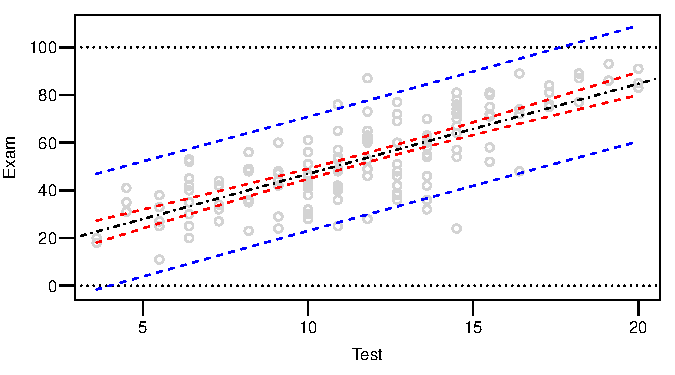
\includegraphics{figure/RC-H02-037}
\end{figure}

\end{frame}



%%%%%%%%%%%%%%%%%%%%%%%%%%%%%%%%%%%%%%%%%%%%%%%%%%%%%%%%%%%%%%%%%%%%%%%%%%%%%%%%%%%%%%%%%%%
\BeginSection{A recipe for subsequent analyses}
%%%%%%%%%%%%%%%%%%%%%%%%%%%%%%%%%%%%%%%%%%%%%%%%%%%%%%%%%%%%%%%%%%%%%%%%%%%%%%%%%%%%%%%%%%%



\begin{frame}[fragile]
\frametitle{A recipe for subsequent analyses}

Here is a recipe (algorithm\footnote{In mathematics and computer science, an algorithm  is a self-contained step-by-step set of operations to be performed. Named after the the mathematician, Mohammed ibn-Musa al-Khwarizmi, who was part of the royal court in Baghdad and who lived from about 780 to 850 AD. }) to use for problems like this where we are interested in a numerical \textbf{response} variable $y$ (e.g.: \rcode{Exam})  and its relationship with a possible \textbf{explanatory} variable $x$ (e.g.:\rcode{Test}):

\end{frame}

\begin{frame}[fragile]
\frametitle{A recipe for subsequent analyses\ldots}

\begin{itemize}
\item Plot the data and see what sort of relation (if any) it suggests (there may also be a statement of research intent to guide you). 
Propose an appropriate working model. 
In the above example we decided that 
$y_i=\beta_0+\beta_1 x_i+\varepsilon_i, \;\;  \varepsilon_i\iid N(0,\sigma^2)$ (where $\beta_1>0$.)

\item Fit the working model using \rcode{lm}.

\item Check the assumptions you are using and validate them. Independence OK? (how were the data collected?), EOV Okay? -- \rcode{plot(examtest.fit, which = 1)}, Normality Okay? -- \rcode{normcheck}. 
If these are okay then,

\item Remove any non-significant explanatory variables where appropriate (more about this later). If so, check new working model.

\item Make sure that individual points are not having undue influence and, perhaps, eliminate/correct them -- \rcode{cooks20x}. If these are okay then,

\item Make conclusions/predictions, discuss limitations, and answer relevant research questions.

\medskip
Note in the above do not  go to the next step until you are satisfied with the current step. 
\end {itemize}

\end{frame}



%\begin{frame}
%\frametitle{Chapter 2 Summary}

%More on the simple linear model: $\E[Y|X]=\beta_0+\beta_{1}X$. 

%For a single observation, $y_i$, the simple linear model is:

%$$ y_i = \beta_0+\beta_{1}x_i + \varepsilon_i.$$

%\begin{itemize}
%  \item The assumptions of 
%\end{itemize}
%and how we assess whether they are satisfied by the data.

%The assumptions:

%\begin{itemize}
  %\item The random errors are iid $N(0, \sigma^2)$. I.e.
  %\begin{enumerate}
  %  \item They are pairwise mutually independent (uncorrelated).
  %  \item They have constant variance, $\sigma^2$, across the all values of the explanatory variable.
  %  \item They are normally distributed with mean 0 and variance $\sigma^2$.
  %  \item There are no outliers.
%  \end{enumerate}
 % \item The assumptions apply to all of the linear models you will encounter in Chapters 1 - 12. 
%  \item To fit in \rcode{R}: \rcode{fit = lm(formula)}, where \rcode{formula = y \textasciitilde{} x}.
%  \item Use \rcode{summary(fit)} to get table of coefficients containing estimates of $\beta_0$ and $\beta_{1}$. 
%  \item Prediction in \rcode{R}: \rcode{summary(fit)}
%  \item We use $R^2$ to assess ``goodness'' of prediction
%\end{itemize}

%\end{frame}


%%%%%%%%%%%%%%%%%%%%%%%%%%%%%%%%%%%%%%%%%%%%%%%%%%%%%%%%%%%%%%%%%%%%%%%%%%%%%%%%%%%%%%%%%%%
\BeginSection{Relevant \rcode{R}-code}
%%%%%%%%%%%%%%%%%%%%%%%%%%%%%%%%%%%%%%%%%%%%%%%%%%%%%%%%%%%%%%%%%%%%%%%%%%%%%%%%%%%%%%%%%%%


\begin{frame}[fragile]
\frametitle{Most of the \rcode{R}-code you need for this chapter}

Fitting a linear (straight line) model to these data.


\begin{knitrout}\scriptsize
\definecolor{shadecolor}{rgb}{0.969, 0.969, 0.969}\color{fgcolor}\begin{kframe}
\begin{alltt}
\hlstd{> }\hlstd{examtest.fit}\hlkwb{=}\hlkwd{lm}\hlstd{(Exam}\hlopt{~}\hlstd{Test,} \hlkwc{data}\hlstd{=Stats20x.df)}
\end{alltt}
\end{kframe}
\end{knitrout}

Note: Independence is evaluated by investigating how the data was collected. Observations are assumed to be acting independently of each other. Much thought must go into making sure this assumption holds.

Checking for EOV

\begin{knitrout}\scriptsize
\definecolor{shadecolor}{rgb}{0.969, 0.969, 0.969}\color{fgcolor}\begin{kframe}
\begin{alltt}
\hlstd{> }\hlkwd{plot}\hlstd{(}\hlkwc{examtest.fit.which}\hlstd{=}\hlnum{1}\hlstd{)}
\end{alltt}
\end{kframe}
\end{knitrout}

Checking approximate normality
\begin{knitrout}\scriptsize
\definecolor{shadecolor}{rgb}{0.969, 0.969, 0.969}\color{fgcolor}\begin{kframe}
\begin{alltt}
\hlstd{> }\hlkwd{normcheck}\hlstd{(examtest.fit)}
\end{alltt}
\end{kframe}
\end{knitrout}

Checking for points of undue influence:

\begin{knitrout}\scriptsize
\definecolor{shadecolor}{rgb}{0.969, 0.969, 0.969}\color{fgcolor}\begin{kframe}
\begin{alltt}
\hlstd{> }\hlkwd{cooks20x}\hlstd{(examtest.fit)}
\end{alltt}
\end{kframe}
\end{knitrout}



\end{frame}

\begin{frame}[fragile]
\frametitle{Most of the \rcode{R} code you need for this chapter...}

Estimated values from the fitted model:

\begin{knitrout}\scriptsize
\definecolor{shadecolor}{rgb}{0.969, 0.969, 0.969}\color{fgcolor}\begin{kframe}
\begin{alltt}
\hlstd{> }\hlkwd{summary}\hlstd{(examtest.fit)}
\end{alltt}
\end{kframe}
\end{knitrout}
Confidence intervals for the model parameters (intercept and slope)

\begin{knitrout}\scriptsize
\definecolor{shadecolor}{rgb}{0.969, 0.969, 0.969}\color{fgcolor}\begin{kframe}
\begin{alltt}
\hlstd{> }\hlkwd{confint}\hlstd{(examtest.fit)}
\end{alltt}
\end{kframe}
\end{knitrout}

Creating a  data frame of new values (for, say,  Test =0, 10 or 20):
\begin{knitrout}\scriptsize
\definecolor{shadecolor}{rgb}{0.969, 0.969, 0.969}\color{fgcolor}\begin{kframe}
\begin{alltt}
\hlstd{> }\hlstd{preds.df}\hlkwb{=}\hlkwd{data.frame}\hlstd{(}\hlkwc{Test}\hlstd{=}\hlkwd{c}\hlstd{(}\hlnum{0}\hlstd{,}\hlnum{10}\hlstd{,}\hlnum{20}\hlstd{))}
\end{alltt}
\end{kframe}
\end{knitrout}
Confidence intervals for expected values and prediction intervals for new observations:
\begin{knitrout}\scriptsize
\definecolor{shadecolor}{rgb}{0.969, 0.969, 0.969}\color{fgcolor}\begin{kframe}
\begin{alltt}
\hlstd{> }\hlcom{# confidence interval for expected value:}
\hlstd{> }\hlkwd{predict}\hlstd{(examtest.fit, preds.df,} \hlkwc{interval}\hlstd{=}\hlstr{"confidence"}\hlstd{)}
\hlstd{> }\hlcom{# prediction interval for new observation:}
\hlstd{> }\hlkwd{predict}\hlstd{(examtest.fit, preds.df,} \hlkwc{interval}\hlstd{=}\hlstr{"prediction"}\hlstd{)}
\end{alltt}
\end{kframe}
\end{knitrout}

\end{frame}

\end{document}


%%%%%%%%%%%%%%%%%%%%%%%%%%%%%%CUT BITS%%%%%%%%%%%%%%%%%%%%%%%%%%%%%%%%%%%%%%%%%%%%%%%%%%%%%%

\begin{frame}[fragile]
\frametitle{Plot layout example}
\begin{knitrout}\scriptsize
\definecolor{shadecolor}{rgb}{0.969, 0.969, 0.969}\color{fgcolor}
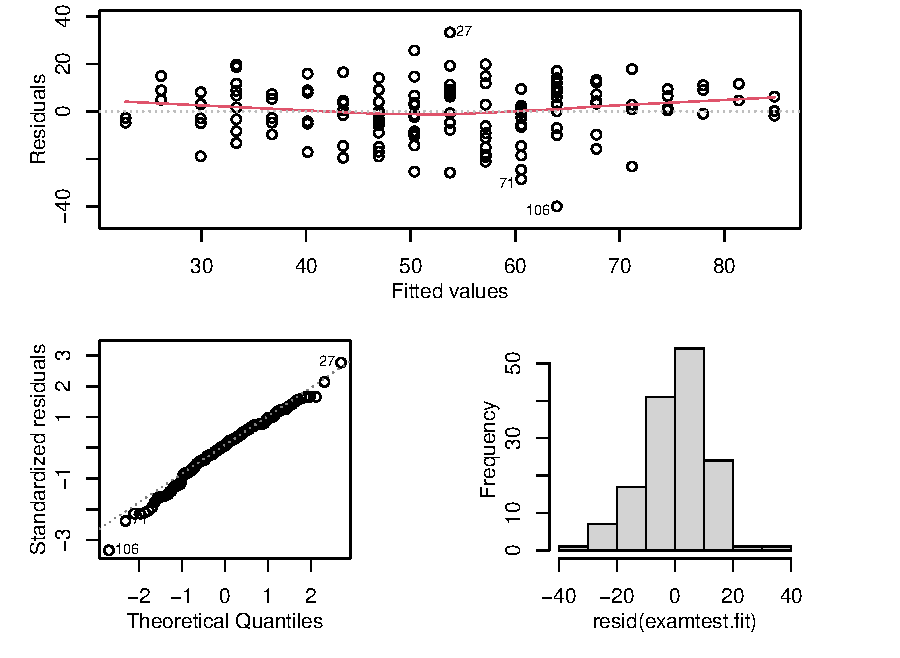
\includegraphics[width=\maxwidth]{figure/Layout_test2-1} 
\end{knitrout}
\end{frame}





\begin{frame}[fragile]
\frametitle{Model assumptions}
\framesubtitle{Garbage in  --  garbage out}


This machinery of least squares assumes that the `fuel' (data) is of a certain standard.
The machinery will still  work (i.e. give output) even if the data does not conform to these standards. 

\medskip

It will, however, probably result in, at least, misleading results and, at most, totally useless results.

\medskip

{\bf\ Ass\textbackslash u\textbackslash me}: if you make assumptions without validating them, you will make an \textbf{Ass} out of \textbf{U} and \textbf{me}!!

\end{frame}

